\documentclass[letterpaper]{article}
\usepackage{uai2019}
\usepackage[margin=1in]{geometry}

% Set the typeface to Times Roman
\usepackage{times}
\usepackage[utf8]{inputenc}
\usepackage{mathtools}
\usepackage{amsfonts}
\usepackage{booktabs}
\usepackage[colorlinks=true,citecolor=blue,urlcolor=blue]{hyperref}

\newcommand{\mean}[1]{\left\langle #1 \right\rangle}
\newcommand{\avg}[1]{\langle#1\rangle}
\newcommand{\et}{\;\mathrm{and}\;}
\newcommand{\Real}{\mathbb{R}}
\newcommand{\STAB}{\mathrm{STAB}}
\renewcommand{\TH}{\mathrm{TH}}

\title{Exclusivity graph approach to Instrumental inequalities}

%\author{Davide Poderini}
%\author{Iris Agresti}
%\author{Gonzalo Carvacho}
%\author{Fabio Sciarrino}
%\affiliation{Dipartimento di Fisica, Sapienza Universit\`{a} di Roma,
%Piazzale Aldo Moro 5, I-00185 Roma, Italy}
%
%\author{Rafael Chaves}
%\affiliation{International Institute of Physics, Federal University of Rio %Grande do Norte, 59070-405 Natal, Brazil}
%\affiliation{School of Science and Technology, Federal University of Rio %Grande do Norte, 59078-970 Natal, Brazil}

\author{} % LEAVE BLANK FOR ORIGINAL SUBMISSION.
          % UAI  reviewing is double-blind.

\begin{document}

\maketitle

\begin{abstract}
Instrumental variables allow the estimation of cause and effect relations even
in presence of unobserved latent factors, thus providing a powerful tool for any
science wherein causal inference plays an important role. More recently, the
instrumental scenario has also attracted increasing attention in quantum
physics, since it is related to the seminal Bell's theorem and in fact allows
the detection of even stronger quantum effects, thus enhancing our current
capabilities to process information and becoming a valuable tool in quantum
cryptography. In this work, we further explore this bridge between causality and
quantum theory and apply a technique, originally developed in the field of
quantum foundations, to express the constraints implied by causal relations in
the language of graph theory. This new approach can be applied to any causal
model containing a latent variable. Here, by focusing on the instrumental
scenario, it allows us to easily reproduce known results as well as obtain new
ones and gain new insights on the connections and differences between the
instrumental and the Bell scenarios. 
\end{abstract}

\section{Introduction}
Inferring  whether a variable $A$ is the cause of another variable $B$ is at the
core of causal inference. However, unless interventions are available
\cite{pearlbook}, one can cannot exclude that observed correlations between $A$
and $B$ are due to a latent common factor, thus hindering any causal
conclusions. To cope with that, instrumental variables (IV) have been introduced
\cite{pearl1995, bonet2001}. Under the assumption that they are independent of
any latent common factors, IV can be used to put non-trivial bounds on the
causal effect between $A$ and $B$. To this aim, first, one has to guarantee that
an appropriate instrument (fulfilling a set of causal constraints) has been
employed, which is precisely the goal of the so-called instrumental tests
\cite{pearl1995, bonet2001}. Their violation, at least in classical physics, is
an unambiguous proof that some of the causal assumptions underlying the
instrumental causal structure are not fulfilled, that is, one should identify
and use another instrumental variable.

The first instrumental tests have been introduced by Pearl \cite{pearl1995}, in
the form of inequalities providing a necessary condition for a given observed
probability distribution to be compatible with the instrumental causal
structure. Following that, Bonet \cite{bonet2001} introduced a general
framework, showing that the instrumental correlations define a polytope, a
convex set from which the non-trivial boundaries are precisely the instrumental
inequalities. Bonet's framework allows for the derivation of new inequalities
as well as proving general results, for instance, the fact that if variable $A$
is continuous, no instrumental test exists. However, two main drawbacks arise. First, the systematic derivation of new inequalities quickly becomes
unfeasible as the variables' cardinalities increase. Second, as recently shown,
in quantum physics, violations of the instrumental tests are possible even
though the whole process is indeed subjected to an instrumental causal structure
\cite{chaves2018, himbeeck2018}. In the quantum case, instrumentality violations
witness the presence of quantum entanglement as the latent factor and prove a
stronger form of quantum non-locality compared to the famous Bell's theorem
\cite{chaves2018}. As a consequence, typical bounds on the causal influence of
$A$ into $B$ have to be reevaluated and reinterpreted in the presence of quantum
effects.

Our aim in this paper is to provide a novel and complementary framework to the
analysis of instrumental tests, which also addresses the two drawbacks mentioned
above. The proposed method is based on a graph theoretical approach introduced
in the foundations of quantum physics to analyze the possible correlations
obtained in quantum experiments \cite{cabello2014,rabelo2014}. This method allow us to reproduce the classical results by Bonet and to straightforwardly generalize them in the quantum scenario. It also offers an easy and general way -- valid for any causal scenario involving a single latent variable-- to check for the incompatibility between the
quantum and classical descriptions.

The paper is organized as follows: first we provide the necessary background for our work, describing the instrumental and Bell scenarios from both classical and quantum perspectives and introducing the exclusivity graph approach. We then show the versatily of our framework by rederiving and generalizing known results in the literature, obtaining new instrumental inequalities that hardly could be found by standard means and offering new insights about the similarities and differences between instrumental and Bell inequalities.

\begin{figure}[t]
    \centering
    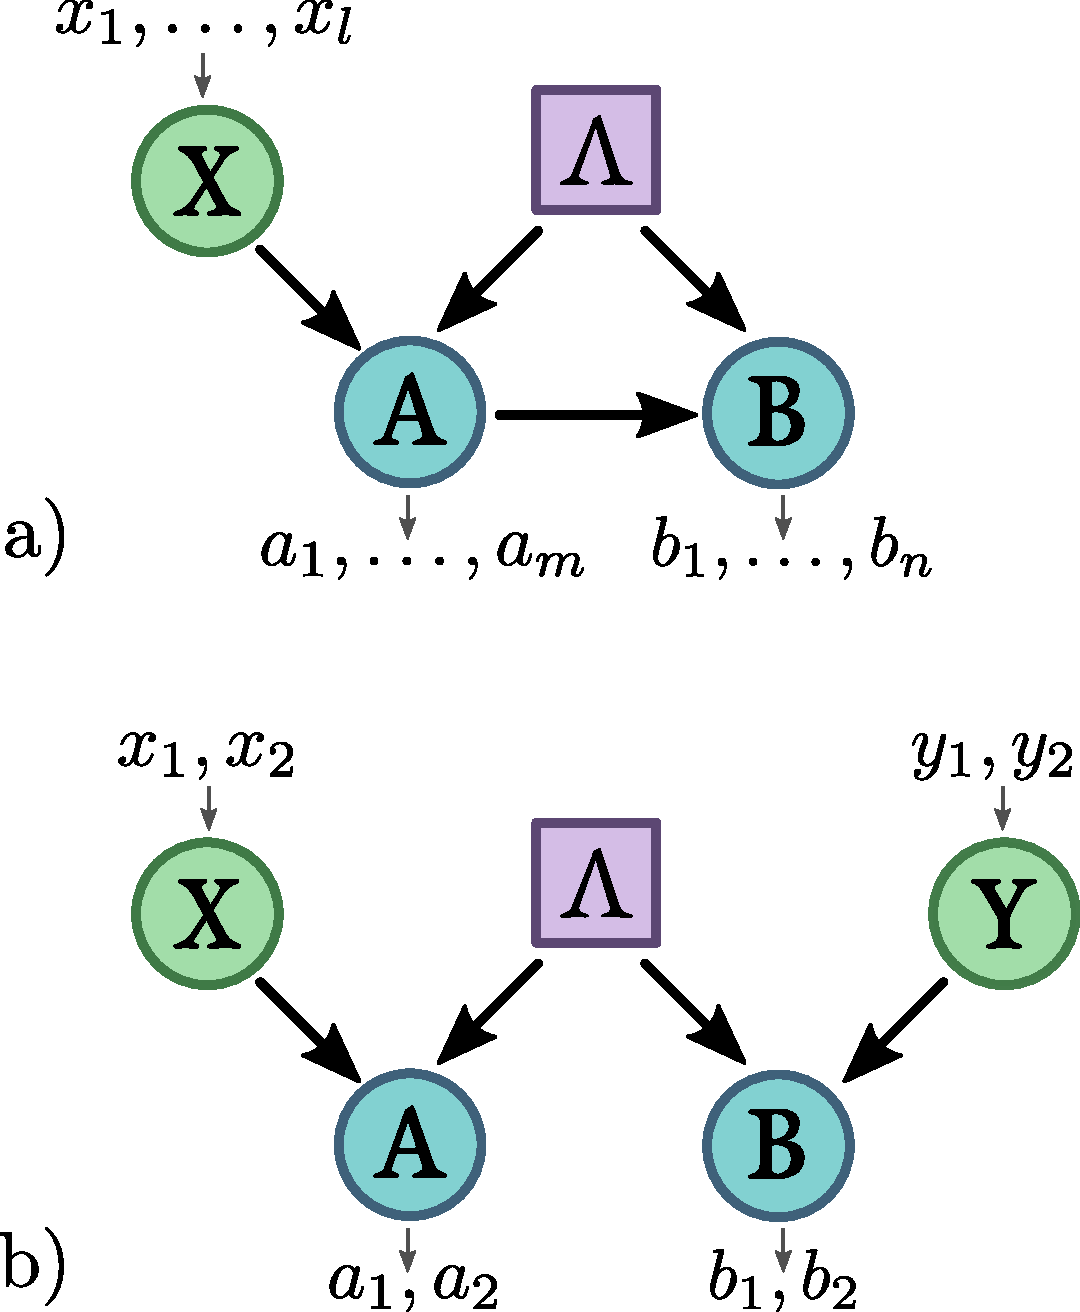
\includegraphics[width=.8\columnwidth]{images/chsh_inst_dag.pdf}
        \caption{
    Directed acyclic graph (DAG) representation for
    \textbf{a)} a general
    Instrumental scenario, with $l$ possible values for the random variable $X$
    and $m,n$ possible outcomes for $A$ and $B$ respectively, and for
    \textbf{b)} the CHSH scenario \cite{CHSH} where all the
    variables $X,Y,A$ and $B$ can only take two possible values.
}
    \label{fig:chshinstdag}

\end{figure} 

\section{Instrumental variables, estimation of causal influences and a new form of quantum non-locality}

It has become standard to represent causal relations via directed acyclic graphs
(DAG), where the nodes represent random variables interconnected by directed
edges (arrows) accounting for their cause and effect relations \cite{pearlbook}.
A set of variables  $\left( X_1,\dots, X_n \right)$ form a Bayesian network with
respect to the graph if every variable $X_i$ can be expressed as a function of
its parents $PA_i$ and potentially an unobserved noise term $U_i$, such that
$U_i$ are jointly independent. This implies that the probability distribution of
such variables should have a Markov decomposition 
\footnote{Uppercase letters label variables and lowercase label the values taken
by them, for instance, $p(X_i =x_i, X_j = x_j) \equiv p(x_i, x_j)$.}
\begin{equation}
p(x_1,\dots,x_n)= \prod_{i=1}^{n} p(x_i \vert pa_i).    
\end{equation}
Importantly, a DAG typically implies non-trivial constraints over the
probability distributions that are compatible with it. That is, simply from
observational data and without the need of interventions, one can test whether
some observed correlations are incompatible with some causal hypotheses.

%and the edges the cause-effect relationship between them.
%From some causal DAGs it is possible to derive constraints on the statistical
%distribution of the variables which allow one to reject or accept a causal
%assumption\cite{pearlbook}.

Within this context, an important DAG is that corresponding to the instrumental
scenario (see Fig.\ref{fig:chshinstdag}-a). Following the Markov decomposition, any
empirical data encoded in the probability distribution $p(a,b \vert x)$ and
compatible with the instrumental causal structure can be decomposed as
\begin{equation}
p(a,b \vert x) = \sum_{\lambda} p(a\vert x,\lambda) p(b\vert a,\lambda)p(\lambda).
\end{equation}
Two causal assumptions are employed to arrive to the above decomposition. First,
the assumption that $p(x,\lambda)=p(x)p(\lambda)$, which implies the independence of
the instrument and the common ancestor. Second, the assumption that, even though
$X$ and $B$ can be correlated, all these correlations are mediated by $A$. In
other terms, there is no direct causal influence between $X$ and $B$ and
$p(b\vert x,a,\lambda)=p(b\vert a,\lambda)$.

The instrumental variables have been originally introduced to estimate parameters
in econometric models of supply and demand \cite{economic} and, since then, have found a
wide range of applications in various other fields \cite{economic2, economic3}. To illustrate its
power, consider that variables $A$ and $B$ are related by a simple structural
equation, i.e. $B=\gamma A +\Lambda$, where $\Lambda$ may represent a latent common
factor. By assumption, the instrumental variable $X$ should be independent of
$\Lambda$, thus implying that the causal strength can be estimated as $\gamma=
\mathrm{Cov}(X,B)/\mathrm{Cov}(X,A)$ where $\mathrm{Cov}(X,A)= \mean{X,A} -
\mean{X}\mean{A}$ is the covariance between $X$ and $A$. Strikingly, one can
estimate the causal strength even without any information about the latent
factor $\Lambda$. More generally, and without assumptions about the functional
dependence among the variables, the empirical data encoded in the probability
distribution $p(a,b \vert x)$ can also be used to bound different quantifiers of
causality between $A$ and $B$ \cite{pearlbook,Janzing2013}.

%Among all the possible causal structures, a
%particular interest has been devoted to the %\textit{Instrumental causal
%structure} (see Fig.\ref{fig:chshinstdag}-a) introduced by Pearl\cite{pearl1995}
%in the 90's with applications ranging from econometrics[] to clinical trial[]. 
%One of the most important properties of instrumental variables is the fact that
%allow us to bound causal relations between variables solely from observational
%data. 
%Like in the Bell tests where the inequalities allow us to test local-realism for
%a particular distribution, instrumental inequalities test whether we have a
%valid instrument.
%Recently has been experimentally proved that instrumental inequalities are also
%violated when considering quantum resources \cite{chaves2018}, thus opening
%several venues for future research such as device-independent cryptography [],
%random number generation[] and basically any application that until now has been
%linked with the Bell scenario.
%In light of the importance regarding the instrumental causal structure, we are
%interested in exploring new techniques in order to better address the question
%of whether we can obtain a quantum violation, and what is the optimal test
%constrained on given experimental data.  

%Let us consider the intrumental structure depicted in Fig.\ref{fig:instdag}
%where X corresponds to the instrument, A and B the variables for which we are
%interested to bound the causal relation and $\Lambda$ our %quantum resource. 

Clearly, however, to draw any causal conclusions, first it is necessary to
certify that one has a valid instrument. This is achieved via instrumental
inequalities, first introduced by Pearl \cite{pearl1995}. If we allow the variables $X$,
$A$, $B$ to take the values in the range  $x=1,\dots,l$, $a=1,\dots,m$ and
$b=1,\dots,n$ Pearl showed that the instrumental causal structure implies that 
\begin{equation} 
    \sum_{j=0}^{n} P(a_i b_j|x_{k(i,j)}) \le 1,
    \label{eq:pearl_ineq}
\end{equation}
for all $i \in {1,\ldots, m}$ and for all the possible functions $k(i,j)$ where $p(a=i,b=j\vert x=k)=p(a_i,b_j|x_k)$.

Extending these results, Bonet \cite{bonet2001} provided a 
general geometric framework for the derivation of instrumental inequalities.
Instrumental correlations define a convex set, a polytope described by finitely
many extremal points, or alternatively by a finite number of facets, among which, the
non-trivial are precisely the instrumental inequalities. In particular,
considering the case $(l,m,n) = (3,2,2)$, it was proven that there are two
inequivalent classes of instrumental inequalities (those not obtained from each
other by permuting the labels of $a_i,b_j$ and $x_k$). One class corresponding
to Pearl's inequality \eqref{eq:pearl_ineq} and the other given by
\begin{multline}
    P(a_1 b_1 | x_1) + P(a_2 b_2 | x_1) + 
    P(a_1 b_1 | x_2) +\\+ P(a_2 b_1 | x_2) + 
    P(a_1 b_2 | x_3) \le 2.
    \label{eq:bonet_ineq}
\end{multline}

All these conclusions and results, however, rely on a classical description of
causal and effect relations, that since Bell's theorem \cite{bell1964} we know do not apply to the world governed by quantum mechanics. This has motivated the
question of whether many of the cornerstones in causal inference have to
reevaluated or reinterpreted in the presence of quantum effects \cite{ried2015,Costa2016}. Indeed, as recently shown \cite{chaves2018}, violations of the instrumental tests are possible even though the causal constraints underlying the instrumental scenario
are fulfilled. As shown in the experimental implementation of the instrumental
test \cite{chaves2018}, this is possible due to the presence of quantum entanglement acting as latent common ancestor.

Interestingly, it has been shown \cite{himbeeck2018} that every probability distribution violating a Bell inequality in the CHSH scenario \cite{CHSH} can after some post-processing also violate Bonet's inequality. The underlying causal structure in a Bell scenario is shown in Fig. \ref{fig:chshinstdag}. It is similar to the instrumental case with two crucial causal differences: i) variable $A$ has no causal influence over $B$ and ii) $B$ has its own instrument $Y$ and thus the correlations are encoded in a probability distribution $p(ab \vert xy)$. As we will see, the graph-theoretical approach will allow us a more systematic understanding of the similarities and differences between the Bell and instrumental scenarios.

%Considering an entangled sources of photons, an alternative version of Bonet's inequality (written in terms of expectation values, upper bounded by 3, in the classical realm) has been tested, implying a violation of the inequality \eqref{eq:bonet_ineq} with a 
%value of $3.258 \pm 0.020$ \textcolor{red}{This refers to the inequality in terms of correlations... what is the violation for the Bonet's inequality in terms of probabilities?}. 

Altogether, this shows the necessity of a new unifying framework, not only
considering what are the classical instrumental correlations but as well the
ones achievable if the underlying latent factor might have a quantum origin. In
the following we will achieve that by proposing a graph-theoretical approach to analyze the instrumental inequalities.

%\begin{equation}
%    -\avg{B}_{x_1} + 2 \avg{B}_{x_2} + %\avg{A}_{x_1} - \avg{AB}_{x_1} +
 %  2\avg{AB}_{x_3} \le 3  
  %  \label{eq:rafael_ineq}
%\end{equation}
%achieving a violation of $3.790 \pm 0.013$, translating to a violation of the original inequality \eqref{eq:bonet_ineq} with a 
%value of $2.159 \pm 0.005$. 

\section{The exclusivity graph approach}

The graph-theoretical approach we propose here, was initially developed for the
study of non-contextual inequalities \cite{cabello2014} as well as Bell
non-locality scenarios \cite{acin2015}. 
In this formalism, every possible event, i.e. every possible set of measurement
outcomes $a_1^,\ldots, a_n$ corresponding to given measurement settings
$x_1,\ldots,x_n$ (each of which can be understood as an instrument), is
associated to a vertex in a (undirected) graph $G = (V, E)$. Two vertices $u, v
\in V$ are then connected by an edge $uv \in E$ if and only if they are
exclusive, i.e.  if exists a measurement/instrument that can distinguish between
them. Any linear constraint (like the instrumental inequalities) can be
expressed defining a linear function
\begin{equation}
    I_w(p) = \sum_{\substack{a_1,\ldots,a_n\\x_1,\ldots,x_n}}
w_{\substack{a_1,\ldots,a_n\\x_1,\ldots,x_n}} p(a_1,\ldots,a_n|x_1,\ldots,x_n)
\end{equation}
on the probabilities of possible events. This linear function can be represented
by the weighted exclusivity graph $G$. Nicely, as it will be discussed below,
bounds for the maximum values for $ I_w(p)$ achievable in classical and quantum
physical theories can be related to two well-known graph invariants \cite{cabello2014}: the
independence number $\alpha(G, w)$ and the Lovász theta $\theta(G, w)$,
respectively. In the following, we will briefly introduce these concepts and
their interconnections, a more extensive and detailed account can be found in
\cite{cabello2014,rabelo2014,acin2015}

Consider a graph $G(V,E)$ with vertex weights $w$, and $|V| = n$ .
We call a \emph{characteristic labelling} for $U \subseteq V$ a vector $x_v \in
\{0,1\}^n$ such that $x_v = 1$ if $v \in U$ and $x_v = 0$ otherwise.

An \emph{independent set} or \emph{stable set} is a set
$S \subset V$ such that $uv \notin E$ for all $u,v \in S$.
The independence number $\alpha(G, w)$ is defined as the maximum number of
vertices (weighted with $w$) of an independent set of $G$. Is also customary to
define the set $\STAB(G)$ as the convex hull of all the
characteristic labelings of stable sets:
\begin{equation} 
    \STAB(G) = \{x : x \quad \text{is a stable labelling of}\quad G \}.
    \label{eq:stab}
\end{equation}
Using this definition the independence number becomes:
\begin{equation}
    \alpha(G,w) = \max\{w\cdot x: x \in \STAB(G)\}
    \label{eq:alphastab}
\end{equation}
From these definitions, we can see that $\alpha(G,w)$ corresponds to the classical bound of the inequality, since it is exactly the maximum over the convex set defined by all the deterministic strategies respecting the exclusivity constraints.

We now call an \emph{orthonormal labelling} of dimension $d$ a map
$a_v:V \rightarrow \Real^d$ such that $a_v \cdot a_u = 0$ for all $uv \in E$ and
$|a_v|^2 = 1$, and we define the set $\TH(G)$ as:
\begin{multline}
    \TH(G) = \{x: x_v = (a_v)_1 \, \text{where $a_v$ is an} \\ \text{orthonormal labelling of $G$}\}
    \label{eq:thbody}
\end{multline}
It can be proved that this set includes all correlations permitted by quantum
theory \footnote{As proved in \cite{acin2015} this set corresponds to the level
$1+AB$ of the NPA (Navascués-Pironio-Acín) hierarchy \cite{npa2008}.}, 
but in general is larger as it contains correlations beyond those achieved by quantum
mechanics \cite{almostquantum2015}.
Maximizing over $\TH(G)$ gives the Lovász theta:
\begin{equation}
    \theta(G,w) = \max \{w\cdot x : x \in \TH(G)\}
    \label{eq:lovasztheta}
\end{equation}
which upper-bounds the maximum quantum value.
This approach provides a useful condition to check if a given graph $G$ admits a
quantum violation. Indeed it can be proven that $\TH(G) = \STAB(G)$ if and only
if $G$ does not contain a cycle $C_n$ with $n \ge 5$ and odd, or its complement
as an induced subgraph. 
This follows directly from the notorious ``sandwich theorem''\cite{knuth,lovasz} and the ``strong
perfect graph theorem'' \cite{spgth}.
The first one states that the number $\theta(G)$ is always ``sandwiched''
between the independence number of the graph $\alpha(G)$ and another quantity
called the \emph{chromatic number} $\chi(G)$, i.e. the smaller number of colors needed
to label the vertices such that vertices connected by and edge always have
different colors.
\begin{equation}
    \alpha(G) \le \theta(G) \le \chi(G)
    \label{eq:sandwich_th}
\end{equation}
When equality holds in equation \eqref{eq:sandwich_th} for a graph $G$ and all its
induced subgraphs, $G$ is called \emph{perfect}.
For perfect graph we can definitely exclude the existence of a quanutm
violation, since $\alpha(G) = \theta(G)$.
The second theorem then gives a useful condition to check if a graph is perfect
or not.  In particular it affirms that a graph $G$ is perfect if and only if it
does not contain a $n$-cycle graph with $n\ge5$ and odd or its complement as an
induced subgraph.

Besides signaling the presence of a possible quantum violation of a classical
constraint, induced cycle subgraphs are also experimentally interesting because
they give the simplest inequalities (in terms of number of probabilities to
estimate), to test this violation.

\section{Exclusivity graph method applied to causal models}
Next we show how the techniques presented in the previous section can be employed to analyze
a broad class of causal models. Consider the DAG depicted in fig~\ref{fig:onelambda}, with
$k$ observable variables $A_k$ with potential causal arrows among them, $l$
instruments $X_l$ with no incoming edges, and a single unobservable latent
variable $\Lambda$ acting as a potential common factor for all $A_k$ (but not to
$X_l$).

\begin{figure}[h]
    \centering
    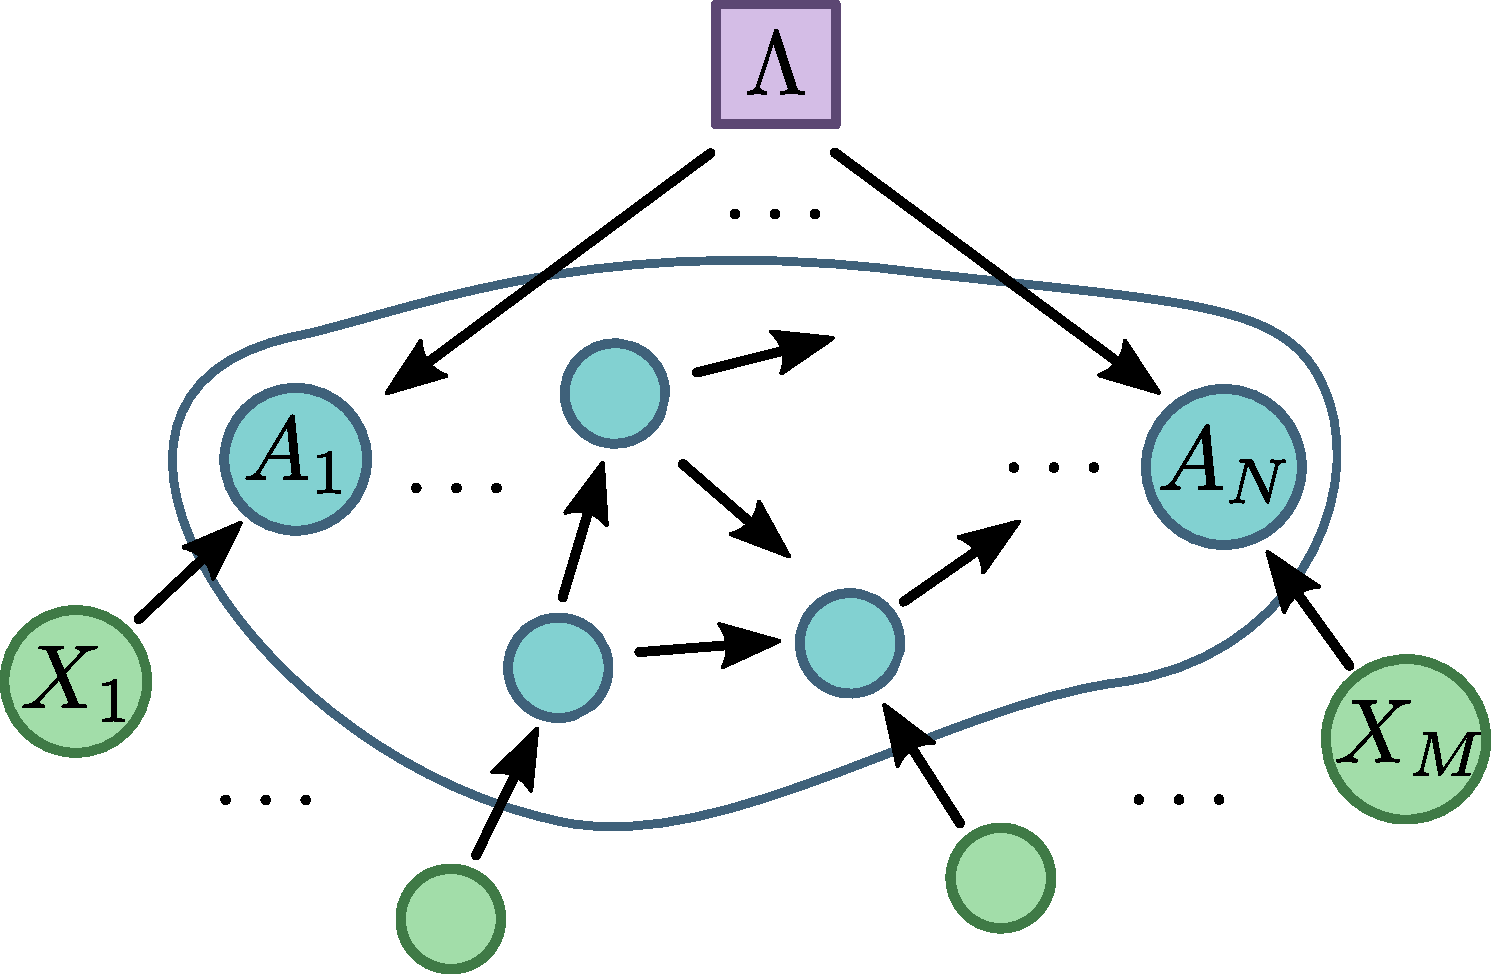
\includegraphics[width=.9\columnwidth]{images/onelambda.pdf}
    \caption{Represetantion of the class of causal structures to which our
        method can be applied, which are those with $k$ observable variables, $l$
        instruments and a single latent variable.}
    \label{fig:onelambda}
\end{figure}

A \emph{non-exclusivity} graph can be associated with such a DAG
%(also called a \emph{confusability} graph) 
as follows:
\begin{itemize}
    \item Nodes are associated to events like $a | x$, where $a = (a_1,\ldots,a_k)$ and  $x = (x_1,\ldots,x_l)$.
    \item Two nodes $a | x $, and $a' | x'$ are linked by an edge if and only if 
        \begin{enumerate}
            \item for all $i,j \in \{1 ,\ldots,k\}$ if $A_i\,
                \rightarrow\, A_j$ then $\exists g_{ij} : g_{ij}(a_i) = a_j
                \et g_{ij}(a'_i) = a'_j$.
            \item for all $i\in \{1,\ldots,l\}$ and $j\in \{1,\ldots,k\}$ if
                $X_i\,\rightarrow\,A_j$ then $\exists f_{ij} : f_{ij}(x_i) = a_j
                \et f_{ij}(x'_i) = a'_j$.
        \end{enumerate}
\end{itemize}

As we will show next, considering the particular case of the instrumental
scenario \cite{pearl1995, bonet2001}, one can apply the graph-theoretical methods delineated before
to the complement of this graph, $G=\bar{G}$, and its subgraphs. This allows to
obtain instrumental inequalities and their respective quantum and
classical bounds.

\subsection{The Instrumental exclusivity graph}
\begin{figure}[t]
    \centering
    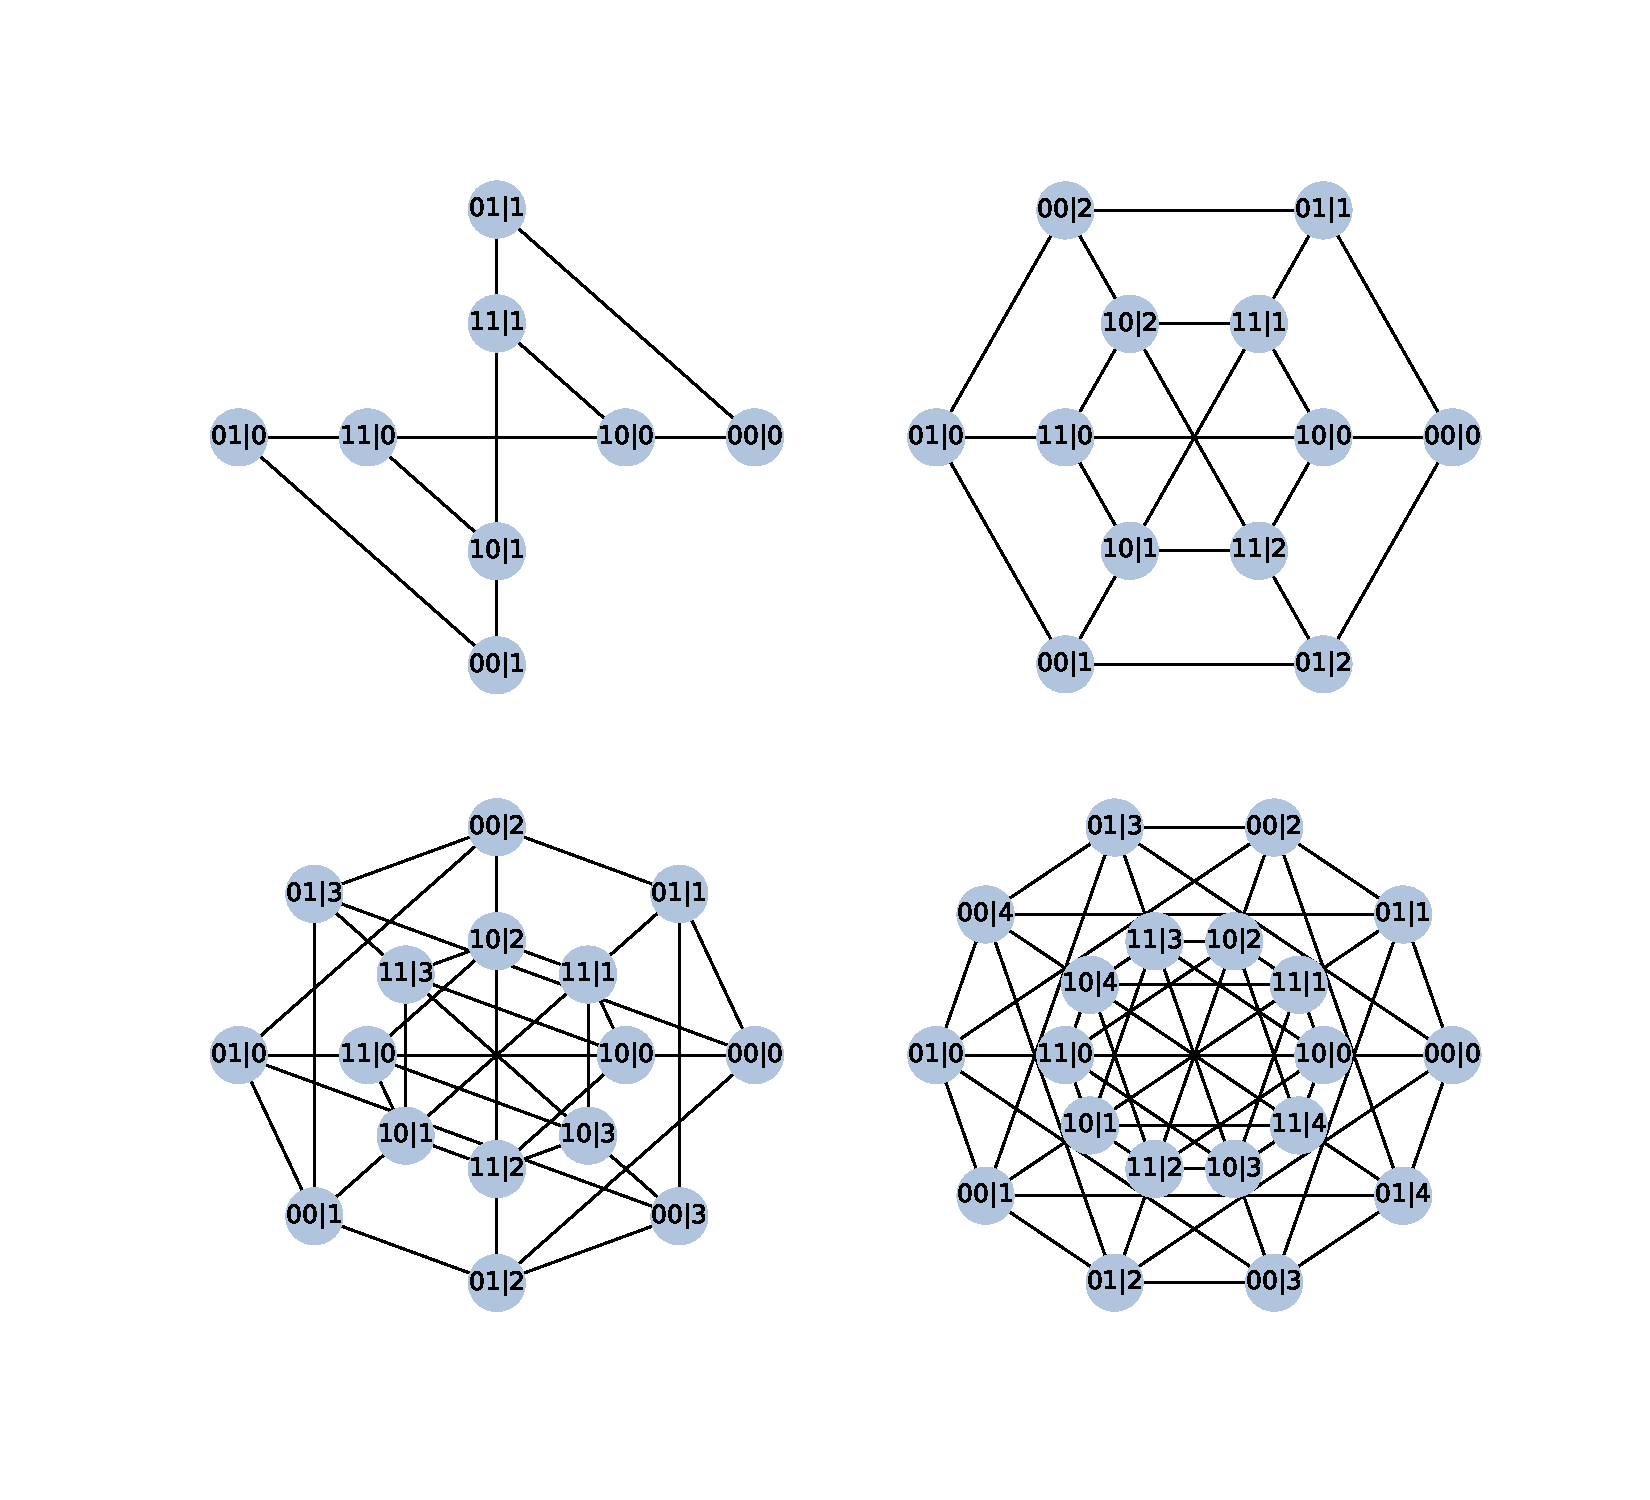
\includegraphics[width=\columnwidth]{images/instrumental_exgraph.pdf}
    \caption{
    The exclusivity graph for the instrumental scenario with $m = n =2$ and $l=2,3,4,5$
    respectively from top left to bottom right. 
    To simplify the representation cliques are represented with the bold lines
    in the figure.}
    \label{fig:instrumental_exgraphs}
\end{figure}

As a first application we will restrict our attention to the case of
dichotomic observables ($n = m = 2$), considering $p(ab|x)$ with $a, b \in
\mathcal{A} = \mathcal{B} = \{0,1\}$ and $x \in
\mathcal{X} = \{0,\ldots,l\}$, the probability of having outcomes $a$ and $b$
with the instrument assuming the value $x$. As detailed above, the
non-exclusivity graph for the instrumental scenario is obtained by linking two
events $ab|x$ and $a'b'|x'$ if there exist two functions $f:\mathcal{X}
\rightarrow \mathcal{A}$ and $g:\mathcal{A} \rightarrow
\mathcal{B}$ such that:
\begin{eqnarray}
   & &  a = f(x) \quad\text{and}\quad a'=f(x')\\ \nonumber
   & & b = g(a) \quad\text{and}\quad b'=g(a')
    \label{eq:non_exclusivity_condition}
\end{eqnarray}
As shown in Fig.~\ref{fig:instrumental_exgraphs}, we construct the exclusivity
graphs for various $l$ and use the methods described earlier to
obtain the classical and quantum bounds for several inequalities in the
instrumental scenario. 

First, consider the case $l=2$, for which Pearl's inequality
\eqref{eq:pearl_ineq} defines the only instrumental inequality. It has been
shown that this inequality does not have a quantum violation \cite{henson2014}.
For that, general probabilistic Bayesian networks, including classical and
quantum causal models as particular cases, had to be introduced.
In contrast, in our method it is straightforward not only to derive the
classical bound to Pearl's inequality but also show that there is no quantum
violation of the inequality. 
Indeed in the case of $l=2$ inequalities \eqref{eq:pearl_ineq} becomes:
\begin{equation}
    P(a0|x_1) + P(a1|x_2) \le 1 
    \label{eq:pearl_ineq_222}
\end{equation}
which are just the classical constraint given by the exclusivity conditions,
represented by the edges of the graph (see Fig.~\ref{fig:instrumental_exgraphs}).
The fact that no quantum violation is allowed follows immediately from the fact
that the corresponding  exclusivity graph (and its complement) does not contain
any odd cycle or anticycle with more than $5$ vertices, which makes it a perfect
graph, i.e. $TH(G) = STAB(G)$. This can be easily generalized to any number of
outputs $n,m$ as shown in the methods section. In this way we can exclude the
presence of any quantum violation for any scenario where the instrument can only
take two possible values ($l=2$) and an arbitrary number of outputs.

\begin{figure}[t]
    \centering
    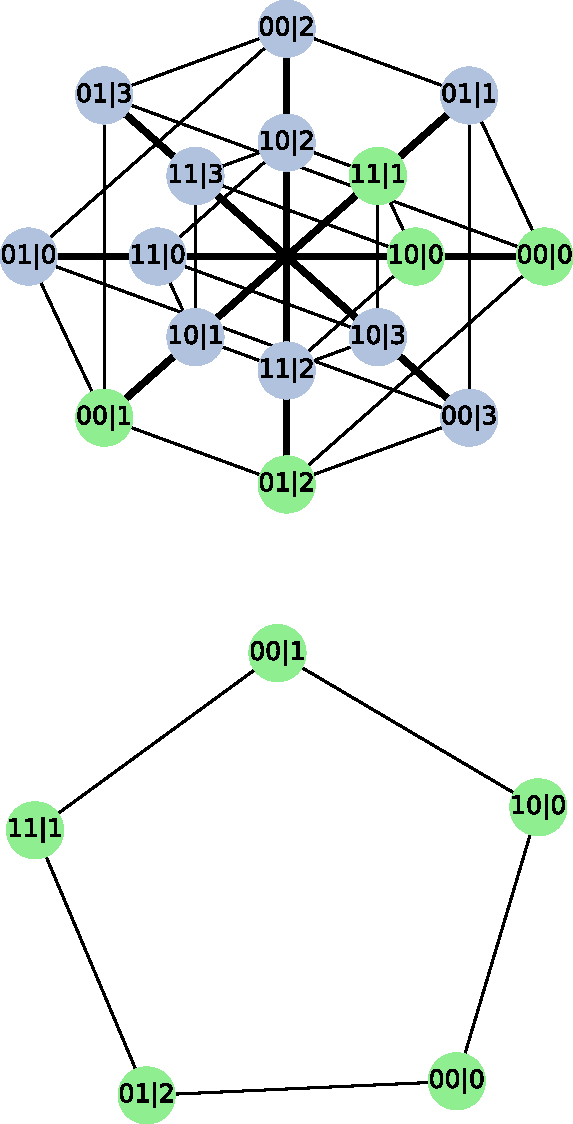
\includegraphics[width=.6\columnwidth]{images/instrumental_c5.pdf}
    \caption{The exclusivity graph of the bonet inequality, as an induced
    subgraph of complete one of the $(l,m,n)=(3,2,2)$ instrumental scenario.To
    simplify the representation cliques are represented with the bold
    lines in the figure.}
    \label{fig:bonetexc}
\end{figure}

Going to $l\ge3$ we see that there might be a quantum violation, since the
associated graph has as a subset a $C_5$ cyclic graph, i.e. the pentagon
depicted in
fig.~\ref{fig:bonetexc} that is exactly the Bonet's inequality \eqref{eq:bonet_ineq}.
For cyclic graphs it is known that $\alpha(C_n) = \lfloor n/2 \rfloor$ and
$\theta(C_n) = n\cos(\pi/n)/(1+\cos(\pi/n))$. For $n=5$, it follows directly the
gap between the classical and quantum theories, since the classical limit is
given by $\alpha(C_5)=2$ and the quantum bound is given by $\theta(C_5)=\sqrt{5}$.

In this framework, Eq. \eqref{eq:bonet_ineq} seems analogous to the KCBS
contextual inequality \cite{kcbs2008} that refers to measurements on single
quantum systems. The difference here is that we are in a bipartite scenario and
the real quantum limit is not simply given by the quantity $\theta(C_5) =
\sqrt{5}$, which constitutes only an upper bound for the maximum achievable
quantum violation. To find a tighter bound we can apply the technique described in
\cite{rabelo2014}, and summarized in the methods sections, based on the NPA
(Navascues, Pironio, Acin) method \cite{npa2008}, in which one defines a hierarchy of
semi-definite programs to progressively compute a better upper bound for the
quantum value.
Applying it to Bonet inequality we are able obtain the known result for the
maximum quantum bound, i.e $(3+\sqrt{2})/2 \approx 2.2071$.

As shown in the Methods section below, no other odd anticycle besides
$C_5$ is present for any $l$, that is, if we increase the cardinality of the
instrumental variable. The first $7$-cycle appears as soon as we get to $n=m=3$ and $l=4$. This Bonet-like inequality for the instrumental scenario can be written as:
\begin{multline}
    P(00|2) + P(02|3) + P(00|0) + P(12|0) + \\
    + P(10|1) + P(21|1) + P(22|2) \le 3 
    \label{eq:c7_instrumental433}
\end{multline}
Applying the method cited above for this inequality gives a quantum upper bound
of $q = 3.2990$ at the second order of the NPA hierarchy, which indicates the
possibility of a quantum violation.
Similarly, numerical analisys shows that odd cycle subgraphs with higher number
of vertices appear only if we increase the number of possible settings $l$ while
also increasing $m$, so for example $9$-cycles start to appear for $l=6, m=3$ 
and $11$-cycles for $l=7, m=4$.

\begin{figure}[t]
    \centering
        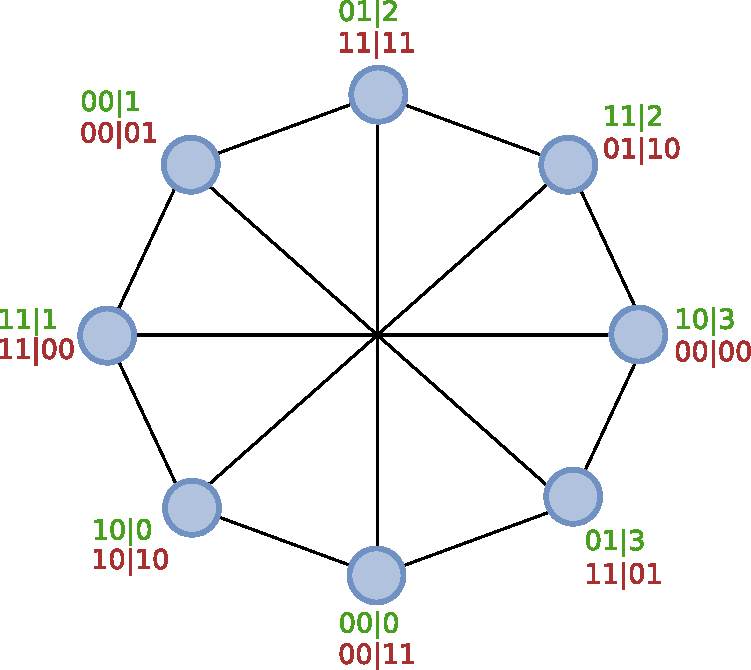
\includegraphics[width=\columnwidth]{images/gclmp_graphs.pdf}
        \caption{Exclusivity graphs for the the inequality \eqref{eq:chsh_ineq} in the Bell
        scenario (in red) and inequality \eqref{eq:422_ineq} in the instrumental
    scenario (in green).}
        \label{fig:422_exgraph}
\end{figure}

While cycles are the simplest inequalities showing quantum violation, our method
can also be employed for the analisys of different inequalities, that can be 
devised by clever choices of vertices and weights. 
For example in the instrumental scenario $(l,m,n) = (4,2,2)$ we can find by inspection the inequality 
%\textcolor{red}{Why are we showing two %inequalities? Aren't they just symmetries of each other?}:

% At first I was showing them because in the standard CHSH 16 probabilities
% appear, 8 with plus and 8 with minus sign, and these probabilities in the
% instrumental mimic the exclusivity relations of the CHSH ones, but you are
% right, is a lot cleaner to just show 8 of them. (Davide)

\begin{multline}
    P(01\vert2) + P(11\vert2) + P(10\vert3) + P(01\vert3) + \\
     + P(00\vert0) + P(10\vert0) + P(11\vert1) + P(00\vert1) \le 3
    \label{eq:422_ineq}
\end{multline}
This inequality is interesting, since it is represented by the same exclusivity graph of the notorious CHSH inequality \cite{CHSH} for the Bell scenario (see Fig.~\ref{fig:422_exgraph}): 
%\textcolor{red}{I'm very confused about these %inequalities... it seems like
%Alice has four %measurement settings... the inequali should be %something like
%$P(00\vert 00) + P(11 \vert 00) + %P(00\vert 01) + P(11 \vert 01) + P(01 \vert
%10) + %P(10 \vert 10) + P(00 \vert 11) + P(11 \vert 11) %\leq 3$, no?}

% Yes of course, sorry, I pasted the wrong one from my notebook... indeed the
% figure shows the one you wrote. (Davide)

\begin{multline}
 P(00\vert 00) + P(11 \vert 00) + P(00\vert 01) + P(11 \vert 01) + \\
 +P(01 \vert 10) + P(10 \vert 10) + P(00 \vert 11) + P(11 \vert 11) \leq 3
\label{eq:chsh_ineq}
\end{multline}

A well known generalization of the CHSH inequality are the so called CGLMP
\cite{cglmp} inequalities, which are defined for any Bell scenario with 2
settings for $X$ and $Y$ and $d$ outputs for $A$ and $B$, and can be written as:
\begin{gather}
    I_d^{\mathrm{CGLMP}} = \sum_{k=0}^{d-1} (d-1-k) S^d_k \le 3 (d-1)\\ \nonumber
    \text{where}\\
    \quad S^d_k = P(b+k,b|00) + P(a, a+k+1|10) +\\ \nonumber
    P(b+k, b | 11) +
    P(a, a+k | 01)
    \label{eq:GCLMP}
\end{gather}
where the sums $a+k, a+k+1$ and $b+k$ are modulo $d$.
Using the exclusivity graph method we can find that each of the $S^d_k$ is
classically constrained by:
\begin{itemize}
    \item $\alpha(G^d_k) = 4$ if $k$ and $d$ satisfy $4k+1=nd$, for some
        integer $n$.
    \item $\alpha(G^d_k) = 3$ in the other cases.
\end{itemize}
Indeed the graphs $G^d_k$ relative to the $k$ all share the same structure:
%represented in Fig.~\ref{fig:gclmp_general},
there are four cliques, one for each setting $x,y \in {0,1}$, and any vertex in each clique is
connected to every other vertex in the adjacent clique, except for one.
For example $P(b+k,b|00)$ is connected to any node belonging to the $(0,1)$ and the
$(1,0)$ cliques, except for $P(a,a+k|01)$ and $P(a',a'+k+1|10)$ where $b+k = a$ and
$a'+k+1 = b$.
Clearly a maximal independent set cannot contain more than $4$ vertices (one for
each clique).
Moreover to be an independent set, a set of four nodes $\{P(b+k,b|00),
P(b'+k,b'|11), P(a,a+k|01), P(a',a;+k+1|01)\}$ must satisfy the conditions:
\begin{equation}
    \left\{
        \begin{aligned}
            &b + k = a \\
            &a + k = b' \\
            &b' + k = a' \\
            &a' + k + 1 = b 
        \end{aligned}
    \right.
    \label{eq:four_indipset_condition}
\end{equation}
where the sums are all modulo $d$.
From this follows directly that $4k+1 = 0$. 

To obtain the quantum bounds we can apply the NPA method as discussed above.
The results for some $S_k$ inequalities are shown in Table~\ref{tab:gclmps}.
%\textcolor{red}{Complete the table or remove it...}
\begin{table}
    \centering
    \begin{tabular}{ccccc}
        $d$ & $k$ & $\alpha(G^d_k)$ & $\theta(G^d_k)$ & NPA \\
        \toprule
         3 & 0 & 3 & 3.464 & 3.333 \\
         3 & 1 & 3 & 3.464 & 3.333 \\
        \midrule
         4 & 0 & 3 & 3.414 & 3.307 \\
         4 & 1 & 3 & 3.414 & 3.307 \\
        \midrule
         5 & 0 & 3 & 3.431 & 3.294 \\
         5 & 1 & 4 & 3.999 & 3.999 \\
        \bottomrule
    \end{tabular}
    \caption{The above table shows the independence number $\alpha(G^d_k)$, the
    Lov\'asz theta $\theta(G^d_k)$, and the NPA bound ,computed to the second
    order of the hierarchy, for the inequalities $S^d_k$ for different values of $k$
    and $d$.}
    \label{tab:gclmps}
\end{table}
        
Interestingly, except for the case $(l,m,n) = (4,2,2)$, inequalities with the
same structure do not seem to arise in the instrumental case, which suggests
that the apparent similarity noticed in \cite{himbeeck2018} between the two scenarios, Bell and the
instrumental, only appears for specific number of inputs and outputs. 

%\section{Finding optimal instrumental inequalities}
%The presence of an odd cycle graph guarantees only that $\STAB(G) \subset
%\TH(G)$, but does not say anything on the %values of $\theta(G)$ and $\alpha(G)$.
%Nonetheless, if that condition is %satisfied there must be some optimal %choice of
%weights $w$ for which we can obtain a %maximum quantum violation.
%Formally if $n$ is the number of nodes of %$G$, we want to find the maximum:
%\begin{equation}
%    \max_{w \in [0,1]^n} \{\theta(G,w) - %\alpha(G,w)\}
%    \label{eq:maxonw}
%\end{equation}
%
%Using the definition \eqref{eq:lovasztheta} and \eqref{eq:alphastab}, and
%remembering that $\STAB(G)$ is a convex %hull of a finite number of
%characteristic labellings we can rewirte %the previous maximization as:
%\begin{align}
%    \Delta &= \min \{I_y : y \, \text{is a %maximal stable labelling}\}
%    \label{eq:maximize_w_delta}\\
%    I_y &= \max_{\substack{w \in %[0,1]^n\\x \in \TH(G)}} \{w\cdot (x - %y)\}
%    \label{eq:maximize_w_I}
%\end{align}
%
%The maximization \eqref{eq:maximize_w_I} %for each $y$ is efficient, being a
%semi-definite program, but unfortunately %it has to be run for each maximal
%stable set in $G$ which are $\sim 3^{n/3}$ %in the worst case.
%Also to enumerate all the maximal %independent sets we used the Tomita %version of
%the Bron–Kerbosch algorithm which has the %same worst case
%complexity\cite{tomita2006}.
%
\section{Discussion}
In this paper, we have proposed an unifying formalism to analyze classical and
quantum correlations arising in a broad class of causal structures. It is based
on a graph-theoretical formalism originally introduced in the field of quantum
information \cite{cabello2014,rabelo2014,acin2015}. In particular, we consider
the application of this formalism to analyze instrumental tests
\cite{pearl1995}. As we show, the probabilities arising in such experiments can
be encoded in a exclusivity graph and from there it follows that the classical
and quantum bounds respected by instrumental inequalities are related to two
graphs invariants: the independence number, $\alpha$, and Lov\'asz $\theta$,
respectively.

Apart from the fundamental relevance of bridging the fields of quantum
information and causal inference, our approach is also shown to be of practical
use. Not only we rederived in an easy manner previous results in the literature,
we also manage to generalize them. For instance, we prove the inequalities
associated with an instrument assuming only two possible values do not have a
quantum violation (irrespectively of the number of outcomes), thus generalizing
the results in \cite{henson2014}. As well, we prove that if the number of
outcomes is fixed to two (the instrument now assuming any cardinality) there no
other inequalities other than the original Bonet's inequality \cite{bonet2001}
that can arise from a n-cycle graph. Following that, we have shown how new
instrumental inequalities associated with n-cycles of increasing n can be
obtained by increasing the possible values of both the instrument and the
outcomes.

The graph approach also constitutes a valuable tool to study similarities among
different scenarios and inspect whether, in the quantum realm, they could be
able to detect stronger forms of non-locality. For example, from the graph
perspective, the instrumental scenario and the well-known Bell scenario shows
similarities only for specific number of inputs/outputs. For example, the CHSH
scenario \cite{CHSH} and the $(l,m,n)=(4,2,2)$ instrumental scenario are graph
equivalent, however, this equivalence does not hold any longer when the outcome
variables assume an increasing number of possible values. Given the fundamental
importance of the instrumental scenario in causal inference and the increasing
attention it has been receiving in quantum information (particularly in
applications as randomness generation) we hope these results will strength the
connections between both fields and motivate further applications of the
graph-theoretical approach within causality.


 %Besides its practical usefulness, this approach constitutes a valuable tool to
 %study similarities among different scenarios and inspect whether, in the
 %quantum realm, they could be able to detect stronger forms of non-locality.
 %For example, from our analysis' results, the instrumental scenario and the
 %well-known Bell scenario shows similarities only for specific number of
 %inputs/outputs (for example, the CHSH scenario and the 422 instrumental
 %scenario are perfectly equivalent). This seems to indicate that, unlike
 %previous works suggested \cite{himbeeck2018}, the instrumental inequalities
 %might be able to reveal a different (and perhaps stronger) form of
 %non-locality, with respect to the Bell scenario.

%\subsubsection*{Acknowledgements}
%We acknowledge support from John Templeton Foundation via the grant Q-CAUSAL
%n$^{\circ}$61084 (the opinions expressed in this publication are those of the
%    authors and do not necessarily  the views of the John Templeton
%Foundation). RC acknowledges the Brazilian ministries MEC and MCTIC, funding
%agency CNPq (PQ grants No. 307172/2017-1 and No 406574/2018-9 and INCT-IQ) and
%the Serrapilheira Institute (grant number Serra-1708-15763).

\section*{Methods}
\subsection*{Edge colored multigraph technique for approximating the quantum
bound}
\begin{figure}[t]
    \centering
    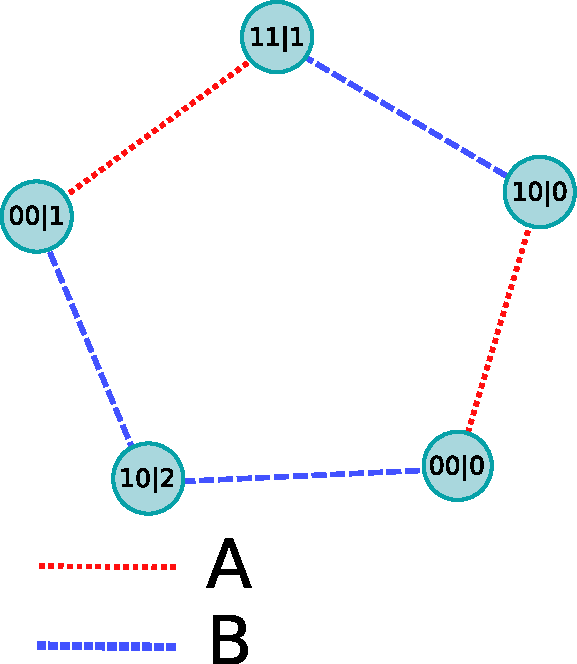
\includegraphics[width=.7\columnwidth]{images/instrumental_multigraph.pdf}
    \caption{Edge colored exclusivity graph representation of the Bonet
        inequality. Exclusivity constraints for the party $A$ and $B$ are
    represented by red lines and blue lines respectively.}
    \label{fig:instrumental_multigraph}
\end{figure}
Applying the technique described above to this scenario yields a quantum
bound of $2.2071$, reproducing the known value for the quantum bound of the Bonet inequality given by $(3+\sqrt{2})/2$.

The Lovasz theta of a graph, despite being efficiently computable, only gives an upper bound to the maximal quantum bound, since it ignores the additional constraints arising from the presence of different parties. To obtain a better approximation for the quantum bound we follow the technique presented
in \cite{rabelo2014}. This method consists in introducing an edge coloring in the exclusivity graph that encodes the information of which of the parties is implying in the given exclusivity constraints under consideration. This effectively corresponds to constructing an exclusivity graph $G_i$ for each
party, the resulting object is called a \emph{multigraph}. Having defined a multigraph $G = {G_1, \ldots, G_n}$ for a given scenario the
quantum bound is defined by the quantity:
\begin{equation}
    \vartheta(G) = \max_{v} \sum_{i \in V} |v \cdot a^1_i \otimes \dots \otimes a^n_i|^2
    \label{eq:multigraph_lovazs}
\end{equation}
where $\{a^j_i\}$ is an orthonormal labelling for $G_j$ and $V$ is the set of vertices of $G$. This quantity, which can be seen as a generalization of the Lov\'asz theta, is in general not efficiently computable, but can be arbitrarily approximated by a hierarchy of semi-definite programs as described in \cite{rabelo2014}.
In the case of the pentagon in the instrumental scenario we have two colors, and thus two graph $G_A$ and $G_B$, corresponding to party $A$ and $B$ respectively, as shown in Fig.~\ref{fig:instrumental_multigraph}.

\subsection*{There are no quantum violation for instrumental scenarios with $l=2$
settings.}
Here we prove that no quantum violation is possible for instrumental scenario
with $l=2$ possible settings for the instrumental variable $X$.
This reduces to proving that there are no odd $n$-cycles nor $n$-anticycles as induced
subgraphs in the corresponding exclusivity graph, with $n\ge5$.
To see this we can notice that any such graph is composed by two cliques (see
for example Fig.~\ref{fig:2mn_nocycle_proof}), corresponding to the events with $x=0$ and
$x=1$.
\begin{figure}[t]
    \centering
    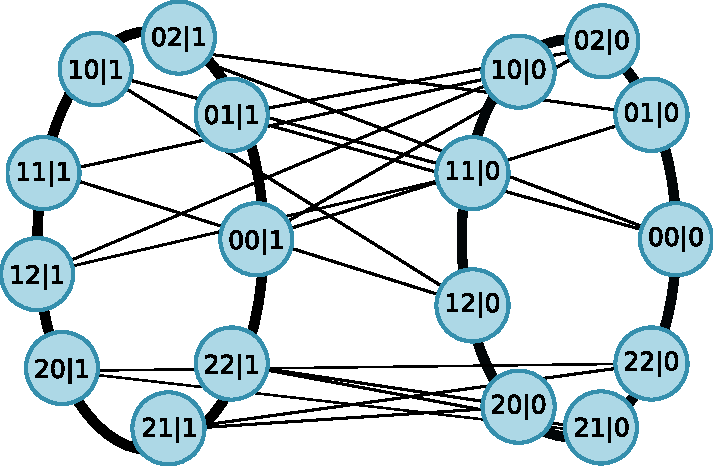
\includegraphics[width=.7\columnwidth]{images/nocycles_proof.pdf}
    \caption{Exclusivity graph for the instrumental scenario $233$, showing the
        impossibility of having cycles with more than $5$ vertices. To simplify the figure cliques are
    represented by bold lines between vertices.}
    \label{fig:2mn_nocycle_proof}
\end{figure}
Any $n$-cycle with at least $5$ vertices must then have at least $3$ mutually
connected vertices belonging to the same $x$, so they can never form a
cycle-graph.
Similarly we can show that there cannot be any induced odd anticycle with $5$ or more
vertices.

\subsection*{There are no cycles $C_n$ with $n \ge 7$ in the $l22$ instrumental scenario.}
%\label{sec:c5only_proof}
In the following we prove that there cannot be a odd anticycle with more than
$5$ vertices in the exclusivity graph associated to an instrumental scenario of
the type $l22$.

\begin{figure}[h]
    \centering
    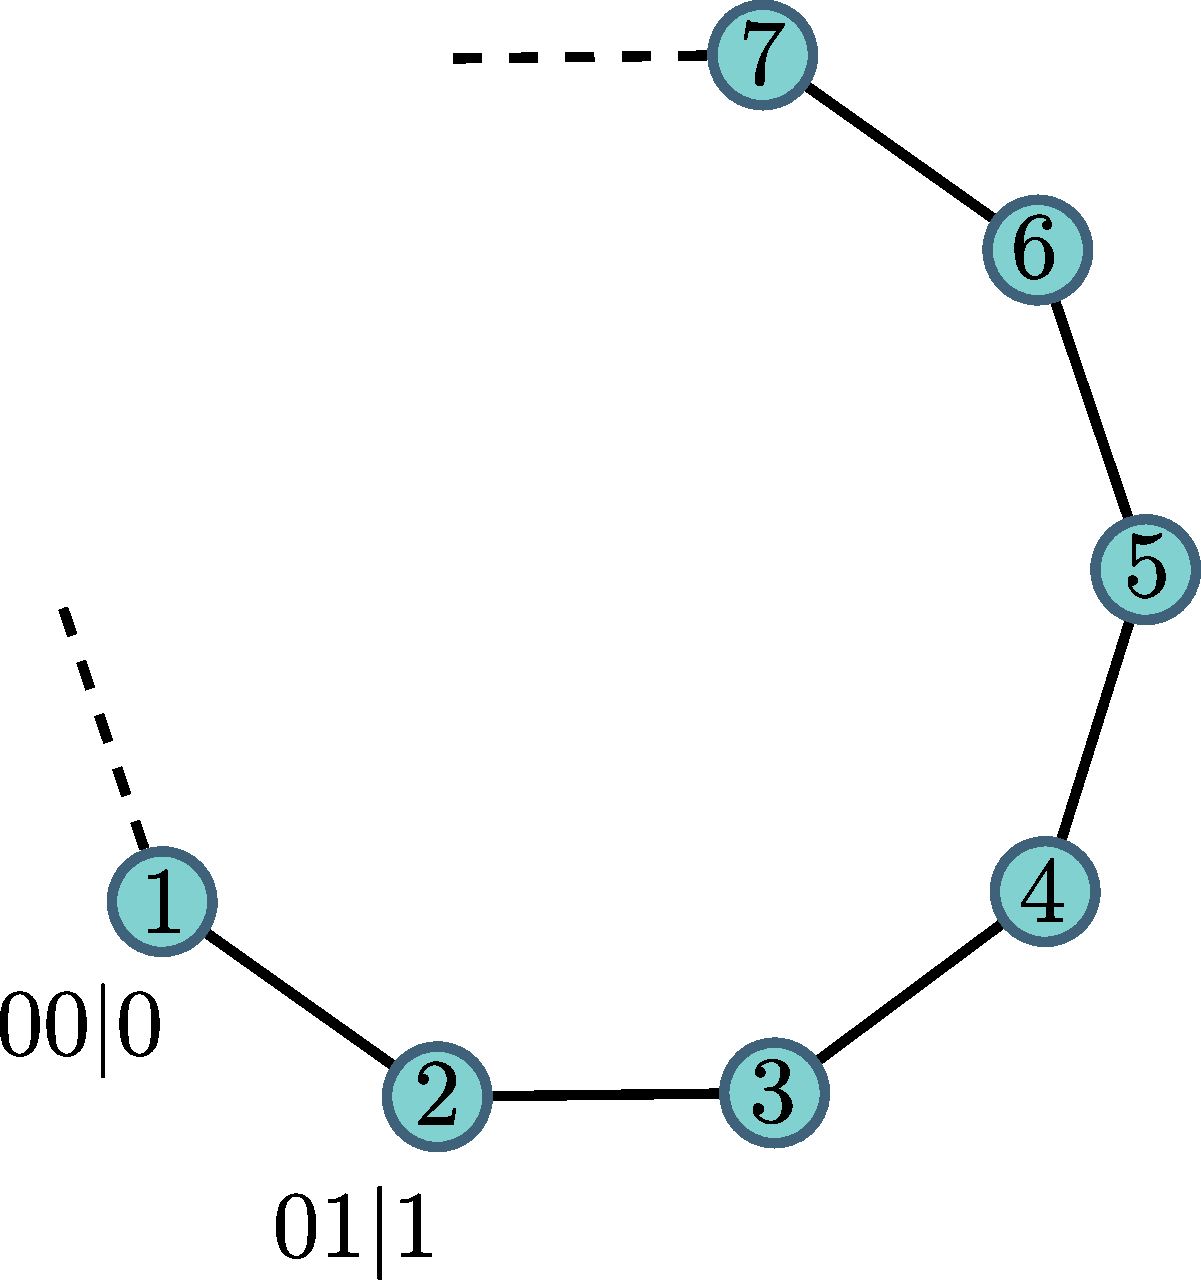
\includegraphics[width=.6\columnwidth]{images/cycle_proof.pdf}
    \caption{Proof of the impossibility of having cycles with $7$ nodes or more
    in the $d22$ scenario.}
    \label{fig:cycle_graph_proof}
\end{figure}

From the exclusivity conditions \eqref{eq:non_exclusivity_condition},
given two events $ab|x$ and $a'b'|x'$, they are connected by edge if one of these two conditions is true:
\begin{enumerate}
    \item $x=x'$.\label{en:rule1}
    \item $a=a'$ and $b \neq b'$.\label{en:rule2}
\end{enumerate}
Suppose we have a cycle $C_n$ with $n \ge 7$, as in fig.~\ref{fig:cycle_graph_proof},
and consider that node $2$ in this graph corresponds to an event which we can arbitrarily identify as $00|0$.
Among its neighbors $1$ and $3$, one will necessarily need to satisfy rule
\ref{en:rule2} (they cannot both satisfy rule \ref{en:rule1} or the three nodes
would be a clique 
%TODO: Explain what is a clique.
So without loss of generality we can assign the event $01|1$ to $3$.
Since nodes $5,6,7$ must not satisfy rule \ref{en:rule2} with both $2$ and $3$, then they must have $a = 1$.
Moreover $7$ and $5$ must have the same $b$, different from $6$. In the same way $1$ must not satisfy rule \ref{en:rule2} with $6,5$ and $3$, so it
needs to have $a=0$ and $b=1$. At this point, since we only have values
$\{0,1\}$ for $a$, we cannot avoid node $4$ to be linked to one of the nodes
$1,2,6,7$. Thus, the corresponding graph cannot be a cycle.

\begin{thebibliography}{}
    \bibitem{pearlbook} J. Pearl, 
        {\em Causality: models, reasoning, and inference.}
        Cambridge University Press, (2000).
    \bibitem{pearl1995} J. Pearl, 
        {\em On the testability of causal models with latent and instrumental variables}, 
        Proceedings of the Eleventh conference on Uncertainty in artificial
        intelligence. Morgan Kaufmann Publishers Inc. (1995).
    \bibitem{bonet2001} B. Bonet, {\em Instrumentality tests revisited},
        Proceedings of the Seventeenth conference on Uncertainty in artificial
        intelligence. Morgan Kaufmann Publishers Inc. (2001).
    \bibitem{chaves2018} R. Chaves, G. Carvacho, I. Agresti, V. Di Giulio, L. Aolita,
        S. Giacomini, F. Sciarrino, 
        {\em Quantum violation of an instrumental test}, 
        Nature Physics 14.3 291 (2018).
     \bibitem{himbeeck2018} T. Van Himbeeck, J. B. Brask, S. Pironio, R. Ramanathan, A. B. Sainz, E. Wolfe, 
        {\em Quantum violations in the Instrumental scenario and their relations to the Bell scenario},
     \bibitem{cabello2014} A. Cabello, S. Severini, A. Winter,
         {\em Graph-theoretic approach to quantum correlations}, 
         Physical review letters, 112, 040401 (2014).
     \bibitem{rabelo2014} R. Rabelo, C. Duarte, A. J.  López-Tarrida, M. T. Cunha, A. Cabello, A. 
         {\em Multigraph approach to quantum non-locality},
         Journal of Physics A: Mathematical and Theoretical, 47, 424021
         (2014).
       \bibitem{CHSH}J.F. Clauser; M.A. Horne; A. Shimony; R.A. Holt, {\em Proposed experiment to test local hidden-variable theories}, Phys. Rev. Lett. 23, 880 (1969).
    \bibitem{economic} P. G. Wright, \emph{The tariff on animal and vegetable oils}, The Macmillan Company, (1928).
    \bibitem{economic2} C. W. J. Granger, \emph{Investigating causal relations by econometric models and cross-spectral methods}, Econometrica, 424 (1969).
    \bibitem{economic3} N. Cartwright, \emph{Causal Structures in Econometrics:On the Reliability of Economic Models},Recent Economic Thought Series \textbf{42}, pp 63-89 (1995).
         \bibitem{Janzing2013} D. Janzing, et al. {\em Quantifying causal influences}, The Annals of Statistics 41, 2324 (2013).
     \bibitem{bell1964} J. S.Bell, {\em On the Einstein Podolsky Rosen Paradox}, Physics 1, 195 (1964).
    \bibitem{ried2015} K. Ried, et al. {\em A quantum advantage for inferring causal structure}, Nature Physics 11, 414 (2015).
     \bibitem{Costa2016}  F. Costa, and S. Shrapnel. {\em Quantum causal modelling}, New Journal of Physics 18, 063032 (2016).
    \bibitem{acin2015} A. Acín, et al. {\em A combinatorial approach to nonlocality and contextuality}, Communications in Mathematical Physics 334, 533 (2015).
     \bibitem{almostquantum2015} M. Navascués, Y. Guryanova, M. J. Hoban, \& A. Acín, {\em Almost quantum correlations.}
         Nature Communications 6, (2015).
     \bibitem{npa2008} M. Navascués, S. Pironio, \& A Acín, 
         {\em A convergent hierarchy of semidefinite programs characterizing the
         set of quantum correlations.}
         New Journal of Physics 10, 073013 (2008).
   \bibitem{knuth} D. Knuth, {\em The sandwich theorem}, The Electronic Journal of Combinatorics 1, 1 (1994).
     \bibitem{lovasz} L. Lovász, 
         {\em An Algorithmic Theory of Numbers, Graphs, and Convexity.}
         CBMS Regional Conference Series in Applied Mathematics (1986), §3.2.
 \bibitem{henson2014} J. Henson, R. Lal, M. F. Pusey. {\em Theory-independent limits on correlations from generalized Bayesian networks}, New Journal of Physics 16, 113043 (2014).
   \bibitem{kcbs2008} A. A. Klyachko, M. A. Can, S. Binicioğlu, A. S. Shumovsky. {\em Simple test for hidden variables in spin-1 systems.}
         Physical review letters, 101(2), 020403 (2008).
   \bibitem{cglmp} D. Collins, et al. {\em Bell inequalities for arbitrarily high-dimensional systems}, Physical review letters 88, 040404 (2002).
     \bibitem{spgth} M. Chudnovsky, N. Robertson, P. Seymour, \& R. Thomas, 
         {\em The strong perfect graph theorem.} 
         Annals of mathematics, 51-229 (2006).
     %\bibitem{tomita2006} E. Tomita, A. Tanaka, \& H. Takahashi,
     %    {\em The worst-case time complexity for generating all maximal cliques
     %    and computational experiments.} 
     %    Theoretical Computer Science 363, 28–42 (2006).
         

%%%%%%%%%%%%%%%%%%%%%%%%%%%%%%%%%%%%%%%%%%%%%%%%%%%%%%%%%%%%%%%%%%%%%%%%%%%% (beta)


%\bibitem{clinical}K. Fischer and I. R. White, \emph{Causal Inference in Clinical Trials}, Wiley-Blackwell, (2012).

%\bibitem{genetic1}N. Friedman, \emph{Inferring cellular networks using probabilistic graphical models}, Science \textbf{303}, 799–805 (2004).

%\bibitem{genetic2}C. R. Shalizi and A. C. Thomas, \emph{Homophily and contagion are generically confounded in observational social network studies}, Sociological methods and research \textbf{40}, 211 (2011).

%\bibitem{social1}H. E. Brady, \emph{Causation and explanation in social science}, Oxford University press (2013).

%\bibitem{machle}D. Barber, \emph{Bayesian reasoning and machine learning}, Cambridge University press (2012).

%%%%%%%%%%%%%%%%%%%%%%%%%%%%%%%%%%%%%%%%%%%%%%%%%%%%%%%%%%%%%%%%%%%%%%%%%%%%%%%%%%

         
         
         
         
         
         
         
%\bibitem{} , {\em },  ().
\end{thebibliography}

%\begin{figure}[h]
%\vspace{1in}
%\caption{Sample Figure Caption}
%\end{figure}

\end{document}
